\section{Algorithmic Components}
\label{sec:algorithmic-components}

\subsection{Instrument Signature Removal}
AUTHOR: Merlin
\begin{itemize}
\item Mask defects and saturation
\item Assembly
\item Overscan
\item Linearity
\item Crosstalk
\item Full frame corrections: Dark, Flats (includes fringing)
\item Pixel level corrections: Brighter fatter, static pixel size effects
\item Interpolation of defects and saturation
\item CR rejection
\item Generate snap difference
\item Snap combination
\end{itemize}

\subsubsection{AP: just skip some steps?}
AUTHOR: Simon

\subsubsection{DRP: do all the steps}
AUTHOR: Merlin


\subsection{Artifact Detection}

\subsubsection{Single-Exposure Morphology}
AUTHOR: Simon
\begin{itemize}
\item Find CRs via morphology.
\item Find satellites via Hough transform.
\item Find some optical ghosts (etc?) from bright star catalog and optics predictions.
\end{itemize}

\subsubsection{Snap Subtraction}
AUTHOR: Simon
\begin{itemize}
\item All of the above, but improve by looking at both snaps.
\end{itemize}

\subsubsection{Warped Image Comparison}
AUTHOR: Jim
\begin{itemize}
\item Find more optical artifacts by looking at differences between warped images (this is run during background matching).
\item Find transient astronomical sources we don't want to include in coadds.
\end{itemize}

\subsection{Artifact Masking/Interpolation}
AUTHOR: Jim
\begin{itemize}
\item Set mask planes for all artifacts.
\item Eliminate small artifacts by interpolating them.
\item Uses PSF model as interpolant.
\end{itemize}

\subsection{Source Detection}
AUTHOR: Jim
\begin{itemize}
\item Detect above-threshold regions and peaks in direct or difference images.
\item Needs to work on preconvolved and unconvolved images.
\item May need multi-pass variants: detect bright objects first, then faint; detect with approximate PSF, then improved.
\end{itemize}

\subsection{Deblending}
AUTHOR: Jim

For templates, try:
\begin{itemize}
\item symmetry ansatz with additional regularization
\item simultaenous fit of galaxy models
\item spline-based models with regularization?
\item (multi-coadd only) optimize color uniformity
\end{itemize}

\subsubsection{Single Visit Deblending}
\begin{itemize}
\item Generate HeavyFootprint deblends using only a single image.
\end{itemize}
\subsubsection{Multi-Coadd Deblending}
\begin{itemize}
\item Generate consistent HeavyFootprint deblends from coadds over multiple bands and possibly epoch ranges.
\end{itemize}

\subsection{Measurement}
AUTHOR: Jim

\begin{figure}
\centering
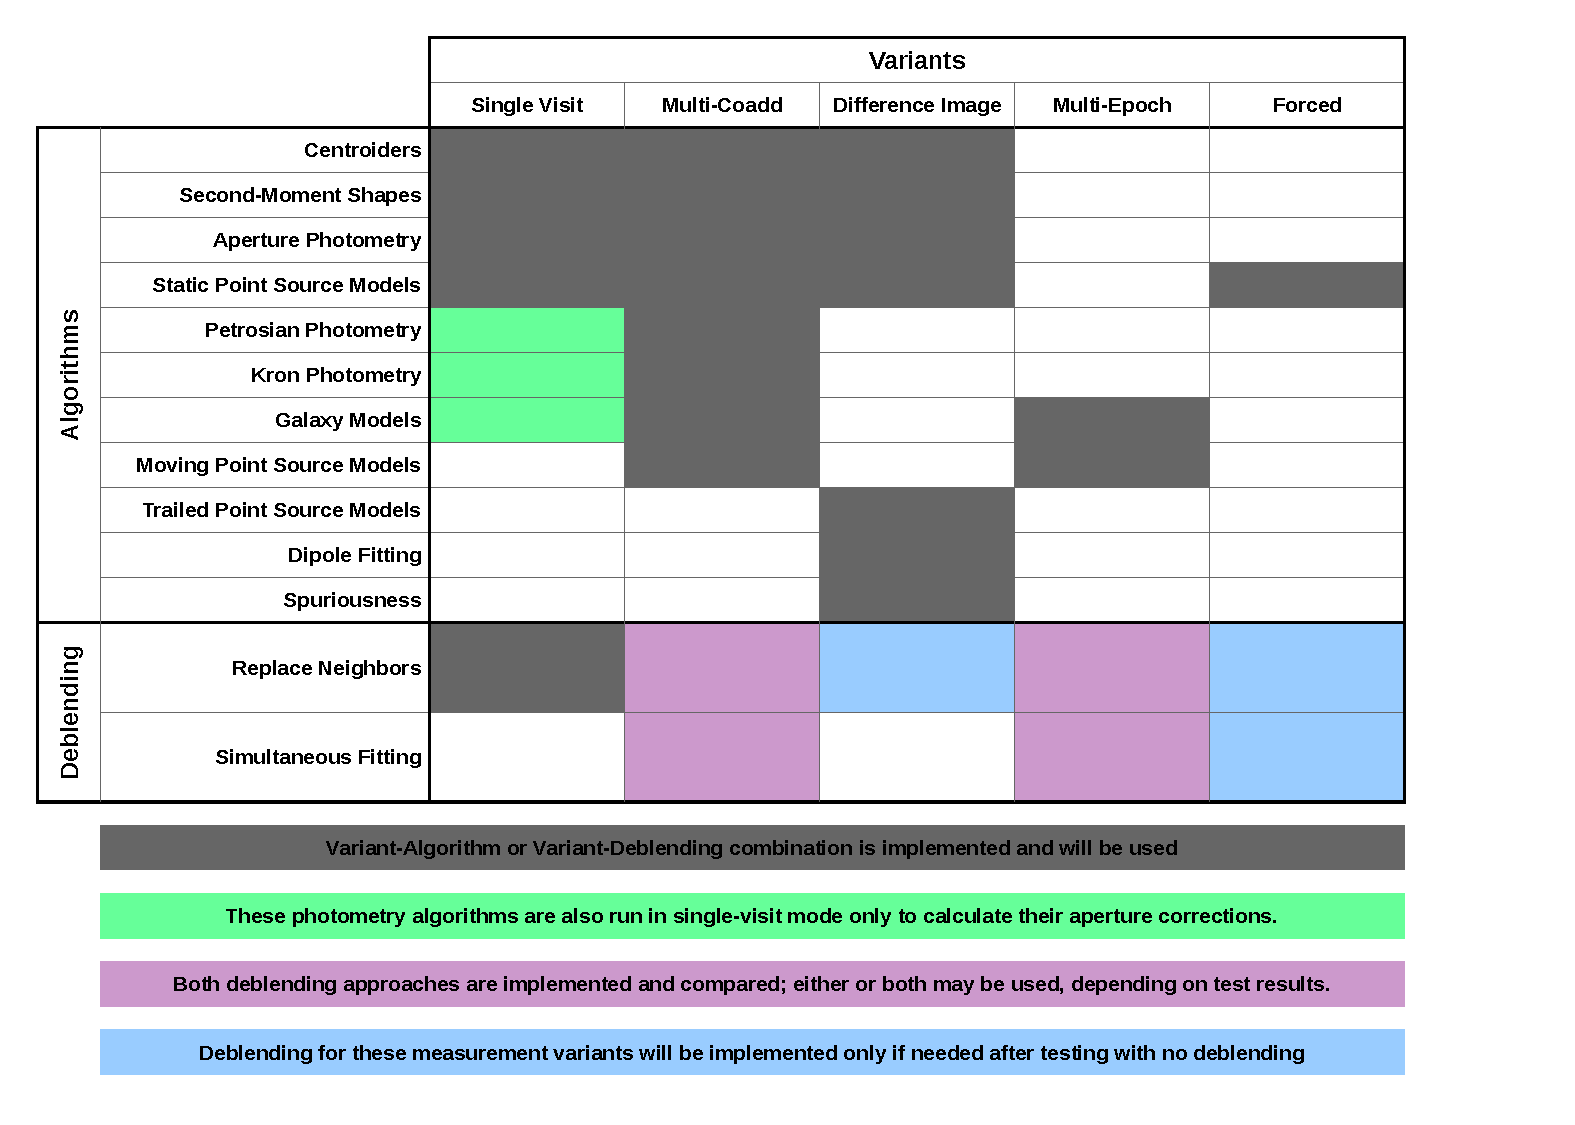
\includegraphics[width=\textwidth]{figures/measurement-matrix.pdf}
\caption{Matrix showing combinations of measurement variants, algorithms, and deblending approaches that will be implemented.
\label{fig:measurement-matrix}}
\end{figure}

\subsubsection{Variants}
Measurement is run in several contexts, but always consists of running an ordered list of algorithm plugins on either individual objects or families thereof.  Each context corresponds to different variant of the measurement driver code, and has a different set of plugin algorithms and approaches to measuring blended objects.

\paragraph{Single Visit Measurement:} Measure a direct single-visit CCD image, assuming deblend information already exists and can be used to replace neighbors with noise (see \ref{sec:blending-replace-neighbors}).

Single Visit Measurement is run in both \hyperref[sec:apSingleFrameProcessing]{AP's Single Frame Processing pipeline}) and DRP's \hyperref[sec:drpBootstrapImChar]{BootstrapImChar}, \hyperref[sec:drpRefineImChar]{RefineImChar}, and \hyperref[sec:drpFinalImChar]{FinalImChar}.

The driver for Single Visit Measurement is passed an input/output \hyperref[sec:spTablesSource]{SourceCatalog} and an \hyperref[sec:spImagesExposure]{Exposure} to measure.  Plugins take an input/output \hyperref[sec:spTablesSource]{SourceRecord} and an \hyperref[sec:spImagesExposure]{Exposure} containing only the object to be measured.

\paragraph{Multi-Coadd Measurement:} Simultaneously measure a suite of coadds representing different bandpasses, epoch ranges, and flavors.  This is run only in DRP's \hyperref[sec:drpMeasureCoadds]{MeasureCoadds} pipeline.

The driver for Multi-Coadd Measurement is passed an input/output \hyperref[sec:spTablesObject]{ObjectCatalog} and a dict of \hyperref[sec:spImagesExposure]{Exposures} to be measured.  Plugins take an input/output \hyperref[sec:spTablesObject]{ObjectRecord} and a dict of \hyperref[sec:spImagesExposure]{Exposures}, each containing only the object to be measured.  Some plugins will also support simultanous measurement of multiple objects, which requires they be provided the subset of the \hyperref[sec:spTablesObject]{ObjectCatalog} to be measured and a dict of \hyperref[sec:spImagesExposure]{Exposures} containing just those objects.

\paragraph{Difference Image Measurement:} Measure a difference image, potentially using the associated direct image as well.  Difference image measurement is run in AP's \hyperref[sec:apAlertDetection]{Alert Detection} pipeline and DRP's \hyperref[sec:drpDiffIm]{DiffIm} pipeline.

The signatures of difference image measurement's drivers and algorithms are at least somewhat TBD; they will take at least a difference image \hyperref[sec:spImagesExposure]{Exposures} and a \hyperref[sec:spTablesSource]{SourceCatalog/SourceRecord}, but some plugins such as dipole measurement may require access to a direct image as well.  Because difference imaging dramatically reduces blending, difference image measurement may require any approach to blended measurement (though any use of the associated direct image would require deblending).

\paragraph{Multi-Epoch Measurement:} Measure multiple direct images simultaneously by fitting the same \hyperref[sec:apWCS]{WCS}-transformed, \hyperref[sec:apPSF]{PSF}-convolved model to them.  Blended objects in Multi-Epoch Measurement will be handled by \emph{at least} fitting them simutaneously (\ref{sec:blending-simultaneous-fitting}), which may in turn require hybrid galaxy/star models (\ref{sec:blending-hybrid-models}).  These models may then be used as templates for deblending and replace-with-noise (\ref{sec:blending-replace-neighbors}) measurement if this improves the results.

Because the memory and I/O requirements for multi-epoch measurement of a single object or blend family are substantial, we will not provide a driver that accepts an \hyperref[sec:spTablesObject]{ObjectCatalog} and measures all objects within it; instead, the \hyperref{sec:drpMultiFit} pipeline will submit individual family-level jobs directly to the orchestration layer.  The multi-epoch measurement driver will thus just operate on one blend family at a time, and manage blending while executing its plugin algorithms.

Multi-epoch measurement for DRP only includes two plugin algorithms, so it is tempting to simply hard-code these into the driver itself, but this driver will also need to support new plugins in Level 3.

Multi-epoch measurement will also be responsible for actually performing forced photometry on direct images, which it can do by holding non-amplitude parameters for moving point-source models fixed and adding a new amplitude parameter for each observation.

\paragraph{Forced Measurement:} Measure photometry on an image using positions and shapes from an existing catalog.

In the baseline plan, we assume that forced measurement will only be run on difference images; while forced photometry on direct images will also be performed in DRP, this will be done by multi-epoch measurement.

Because difference imaging reducing blending substantially, forced measurement may not require any special handling of blends.  If it does, simultaneous fitting (with point-source models) should be sufficient.

The driver for Forced Measurement is passed an input/output \hyperref[sec:spTablesSource]{SourceCatalog}, an additional input \hyperref[sec:spTablesReference]{ReferenceCatalog}, and an \hyperref[sec:spImagesExposure]{Exposure} to measure.  Plugins take an input/output \hyperref[sec:spTablesSource]{SourceRecord}, an input \hyperref[sec:spTablesReference]{ReferenceRecord} and an \hyperref[sec:spImagesExposure]{Exposure}.  If simultaneous fitting is needed to measure blends, plugins will instead receive subsets of the catalogs passed to the driver instead of individual records.

Forced measurement is used by the DRP \hyperref[sec:drpForcedPhotometry]{ForcedPhotometry} pipeline and numerous pipelines in AP.

\begin{note}[TODO]
Add references to specific AP pipelines that will use forced measurement.
\end{note}

\subsubsection{Algorithms}

\paragraph{Centroids}
\begin{itemize}
\item should be equivalent to PSF model fit for stars
\item use larger weight function (TBD) for extended objects
\end{itemize}

\paragraph{Second-Moment Shapes}
\begin{itemize}
\item probably adaptive elliptical Gaussian weights, with fall back to unweightd, PSF-weighted, or some fixed Gaussian
\item add regularization for unresolved objects - avoid crazy ellipticities for objects much smaller than PSF
\end{itemize}

\paragraph{Aperture Photometry}
\begin{itemize}
\item Sequence of fixed apertures
\item Use sinc algorithm for small apertures, naive for large.
\item May use elliptical apertures instead of circular, maybe even if changing ellipticities as a function of radius.  TBD.
\end{itemize}

\paragraph{Static Point Source Models}
\begin{itemize}
\item Fit PSF model for flux only (hold center fixed at centroid or reference value)
\item Doesn't use per-pixel variances for flux measurement, but might also provide measurement with per-pixel variances (for diagnostics?)
\end{itemize}

\paragraph{Kron Apertures}
\begin{itemize}
\item Compute Kron radius (hard to make this robust)
\item Compute flux in elliptical aperture at Kron radius.
\end{itemize}

\paragraph{Petrosian Apertures}
\begin{itemize}
\item Compute Petrosian radius.  Harder than it seems due to need for improvements to splines? (ask RHL)
\item Compute flux in elliptical aperture at Petrosian radius.
\end{itemize}

\paragraph{Galaxy Models}
\begin{itemize}
\item Some sort of bulge+disk model.  Lots of need for experimentation.
\item Will Monte Carlo sample in MultiFit (and maybe on coadds, too, if that helps).
\item May also fit to PSF-matched coadds for consistent colors.
\item Will need to support simultaneous fitting (and sampling).
\item Hybrid model candidate
\end{itemize}

\paragraph{Moving Point Source Models}
\begin{itemize}
\item Fit point source with flux, centroid, parallax, and proper motion parameters.
\item May need to support simultaneous fitting.
\item Might want to sample this too, at least if we fit it simultaneously with sampled galaxy models.
\item Hybrid model candidate
\end{itemize}

\paragraph{Trailed Point Source Models}
\begin{itemize}
\item Fit PSF convolved with line segment to individual images
\end{itemize}

\paragraph{Dipole Models}
\begin{itemize}
\item Fit PSF dipole for separation and flux to a combination of difference image and direct image.
\item Deblending on direct image very problematic.
\end{itemize}

\paragraph{Spuriousness}
\begin{itemize}
\item Some per-source measure of likelhood the detection is junk (in a difference image).
\item May use machine learning on other measurements or pixels.
\item May be augmented by spuriouness measures that aren't purely per-source.
\end{itemize}

\subsubsection{Blended Measurement}
\begin{itemize}
\item Integrate text from blended-measurement doc here.
\end{itemize}

\paragraph{Deblend Template Projection}
\paragraph{Neighbor Noise Replacement}
\label{sec:blending-replace-neighbors}
\paragraph{Simultaneous Fitting}
\label{sec:blending-simultaneous-fitting}
\paragraph{Hybrid Models}
\label{sec:blending-hybrid-models}

\subsection{Background Estimation}
AUTHOR: Simon
\begin{itemize}
\item Fit or interpolate large-scale variations while masking out detections.
\item Needs to work in crowded fields.
\item Needs to work on both difference images and direct images.
\item Need to be able to compose backgrounds measured in different coordinate systems on different scales.
\item Needs to work on single CCDs for AP even if we use full FoV in DRP.
\end{itemize}

\subsection{Build Background Reference}
AUTHOR: Simon
\begin{itemize}
\item Given multiple overlapping visit images (already warped to a common coordinate system), synthesize a continuous single-epoch image that can be used as a reference for background matching.
\end{itemize}

\subsection{PSF Estimation}

\subsubsection{Single CCD PSF Estimation}
AUTHOR: Simon
\begin{itemize}
\item Fit simple empirical PSF model to stars from a single exposure.
\item No chromaticity.
\item May use external star catalog, but doesn't rely on one.
\item Used in Alert Production and BootstrapImChar in DRP.
\end{itemize}

\subsubsection{Full Visit PSF Estimation}
AUTHOR: Jim
\begin{itemize}
\item Decompose PSF into optical + atmosphere.
\item Constrain model with stars, telemetry, and wavefront data.
\item Wavelength-dependent.
\item Used in RefineImChar in DRP.
\item Must include some approach to dealing with wings of bright stars.
\end{itemize}

\subsection{Aperture Correction}
AUTHOR: Jim
\begin{itemize}
\item Measure curves of growth from bright stars.
\item Correct various flux measurements to infinite.
\item Propagate uncertainty in aperture correction to corrected fluxes; covariance is tricky.
\end{itemize}

\subsection{Astrometric Solutions}
AUTHOR: Simon
\subsubsection{Single CCD (for AP)}
\begin{itemize}
\item If this uses DRP's internal reference catalog, this does all we need. THIS IS A NEW DEPENDENCY BETWEEN DRP AND AP.
\end{itemize}
\subsubsection{Single Visit}
\begin{itemize}
\item Fit multi-component WCS to all CCDs in a single visit simultaneously after matching to reference catalog.
\end{itemize}
\subsubsection{Joint Multi-Visit}
\begin{itemize}
\item Fit multi-component WCS to all CCDs from multiple visits simultaneously after matching to reference catalog.
\end{itemize}

\subsection{Photometric Solutions}
AUTHOR: Simon (and Merlin?)
\subsubsection{Single CCD (for AP)}
\subsubsection{Single Visit}
\begin{itemize}
\item Fit zeropoint (and some small spatial variation?) to all CCDs simultaneously after matching to reference catalog.
\item Need for chromatic dependence unclear; probably driven by AP.
\end{itemize}
\subsubsection{Joint Multi-Visit}
\begin{itemize}
\item Derive SEDs for calibration stars from colors and reference catalog classifications.
\item Utilize additional information from wavelenth dependent photometric calibration built by calibration products production.
\item Fit zeropoint and possibly perturbations to all CCDs on multiple visits simultaneously after matching to reference catalog.
\end{itemize}

\subsection{Generate Diffim Template for a Visit}
AUTHOR: Simon
\begin{itemize}
\item Determine appropriate template to use
\item Generate template for observation (may include DCR correction)
\end{itemize}

\subsection{PSF Matching}
AUTHOR: Simon
\subsubsection{Image Subtraction}
\begin{itemize}
\item Match template image to science image, as in Alert Production and DRP Difference Image processing.
\item Includes identifying sources to use to determine matching kernel, fitting the kernel, and convolving by it.
\end{itemize}
\subsubsection{PSF Homogenization for Coaddition}
\begin{itemize}
\item Match science image to predetermined analytic PSF, as in PSF-matched coaddition.
\end{itemize}

\subsection{Image Warping}
AUTHOR: Jim
\subsubsection{Oversampled Images}
\begin{itemize}
\item Just use Lanczos.
\end{itemize}
\subsubsection{Undersampled Images}
\begin{itemize}
\item Can use PSF model as interpolant if we also want to convolve with PSF (as in likelihood coadds).  Otherwise impossible?
\end{itemize}
\subsubsection{Irregularly-Sampled Images}
\begin{itemize}
\item Approximate procedure for fixing small-scale distortions in pixel grid.
\end{itemize}

\subsection{Image Coaddition}
AUTHOR: Jim
\begin{itemize}
\item Can do outlier rejection (but usually doesn't).
\item Needs to propagate full uncertainty somehow.
\item May need to propagate larger-scale per-exposure masks to get right PSF model or other coadded quantities.
\item Should be capable of combining coadds from different bands and/or epoch ranges ranges as well as combining individual exposures.
\end{itemize}

\subsection{DCR-Corrected Template Generation}
AUTHOR: Simon
\begin{itemize}
\item Somwewhat like coaddition, but may need to add dimensions for wavelength or airmass, and may involve solving an inverse problem instead of just compute means.
\end{itemize}

\subsection{Image Decorrelation}
\subsubsection{Difference Image Decorrelation}
AUTHOR: Simon
\begin{itemize}
\item Fourier-space (?) deconvolution of preconvolved difference images before measurement - ZOGY as reinterpreted by Lupton (could apply correction in real space, too)
\item Need to test with small-scale research before committing to this approach.
\end{itemize}

\subsubsection{Coadd Decorrelation}
AUTHOR: Jim
\begin{itemize}
\item Fourier-space/iterative deconvolution of likelihood coadds, as in DMTN-15.
\item Need to test with small-scale research before committing to this approach.
\end{itemize}

\subsection{Star/Galaxy Classification}
AUTHOR: Jim
\subsubsection{Single Visit S/G, Pre-PSF}
\begin{itemize}
\item Select stars to be used in PSF estimation (mostly from moments).
\end{itemize}
\subsubsection{Single Visit S/G, Post-PSF}
\begin{itemize}
\item Extendedness or trace radius difference that classifies sources based on single frame measurements that can utilize the PSF model.  Used to select single-frame calibration stars, and probably aperture correction stars.
\end{itemize}
\subsubsection{Multi-Source S/G}
\begin{itemize}
\item Aggregate of single-visit S/G post-PSF numbers in jointcal.
\end{itemize}
\subsubsection{Object Classification}
\begin{itemize}
\item Best classification derived from multifit and possibly variability.
\end{itemize}

\subsection{Variability Classification}
AUTHOR: John
\subsubsection{Using forced photometry}
\subsubsection{Using DIASources}

\subsection{Proper Motion and Parallax from DIASources}
AUTHOR: Simon

\subsection{Association and Matching}
\subsubsection{Single CCD to Reference Catalog, Semi-Blind}
AUTHOR: Simon
\begin{itemize}
\item Want to match in image coordinates, so also needs to transform reference catalog.
\item Run prior to single-visit WCS fitting, with only telescope's best guess as a starting WCS.
\item Single CCD form needed by AP.
\end{itemize}

\subsubsection{Single Visit to Reference Catalog, Semi-Blind}
AUTHOR: Simon
\begin{itemize}
\item Want to match in focal plane coordinates, so also needs to transform reference catalog.
\item Run prior to single-visit WCS fitting, with only telescope's best guess as a starting WCS.
\end{itemize}

\subsubsection{Multiple Visits to Reference Catalog}
AUTHOR: Jim
\begin{itemize}
\item Match sources from multiple visits to a single reference catalog, assuming good WCSs.
\end{itemize}

\subsubsection{DIAObject Generation}
AUTHOR: Simon
\begin{itemize}
\item Match all DIASources to predicted Solar System object positions and existing DIAObjects and generate new DIAObjects.  Definitely run in AP, maybe run in DRP.
\end{itemize}

\subsubsection{Object Generation}
AUTHOR: Jim
\begin{itemize}
\item Match coadd detections from different bands/SEDs/epoch-ranges, merging Footprints and associating peaks.
\item Also merge in DIASources or (if already self-associated) DIAObjects.
\end{itemize}

\subsubsection{Cross-Patch Merging}
AUTHOR: Jim
\begin{itemize}
\item Resolve duplicates in patch overlap regions by flagging ``primary'' objects.  Difficult due to blending.
\end{itemize}

\subsubsection{Cross-Tract Merging}
AUTHOR: Jim
\begin{itemize}
\item Resolve duplicates in tract overlap regions by flagging ``primary'' objects.  Difficult due to blending.
\end{itemize}

\subsection{Ephemeris Calculation}
AUTHOR: Simon
\begin{itemize}
\item Calculate positions for all solar system objects in a region at a given time.
\end{itemize}

\subsection{Make Tracklets}
AUTHOR: Simon
\begin{itemize}
\item Make all tracklet pairs
\item Merge multiple chained observation into single longer tracklets
\item Purge any tracklets inconsistent with the merged tracklets
\end{itemize}

\subsection{Attribution and precovery}
AUTHOR: Simon
\begin{itemize}
\item Predict locations of known Solar System objects
\item Match tracklet observation to predicted ephimerides taking into account velocity
\item Update SSObjects
\item Possibly iterate
\end{itemize}

\subsection{Orbit Fitting}
AUTHOR: Simon
\begin{itemize}
\item Merge unassociated tracklets into tracks.
\item Fit orbits to all tracks.
\item Purge unphysical tracks.
\item Update SSObjects
\item Possibly iterate
\end{itemize}
